\chapter{Periodic Task Scheduling}
The term task is used to indicate a schedulable entity (either a process or a thread), in particular:
\begin{itemize}
    \item A thread represents a flow of execution (it executes with shared resources, multi thread within the same process)
    \item A process represents a flow of execution + private resources (it executes with its own resources), such as address space, file table, \dots
\end{itemize}

Tasks do not run on bare hardware, but then how can multiple tasks execute on one single CPU?\\
The OS kernel is a piece of the operating system that takes care of multi-programming and somehow it is able to create the illusion that each CPU/processor has its own space, whereas in fact it is sharing the same resources with other processes.\\
In the end the kernel provides the mechanism that enable multiple tasks to execute in parallel; in a sense tasks have the illusion of executing concurrently on a dedicated CPU per task.

On this regard, with the term concurrency we refer to the simultaneous execution of multiple threads/processes in the same PC.\\
Concurrency is implemented by multiplexing tasks on the same CPU. Tasks are alternated on a real CPU and the task scheduler decides which task executes at a given instant in time. In other terms, in order to implement the concurrency mechanism it is necessary to introduce this new component (i.e. the task scheduler), since it makes sure that the time of your pc is shared between the different processes or tasks that compete for the reosurces at that time.

Tasks are associated to temporal constraints (a.k.a. deadlines), hence the scheduler must allocate the CPU to tasks so that their deadlines are respected.

\section{Real Time Scheduling}

\definition{Scheduler}{
    A scheduler generates a schedule from a set of tasks
\begin{enumerate}
    \item In the case of Unicore processor system (UP) (simpler definition), a schedule $\sigma(t)$ is a function mapping time $t$ into an executing task.
    \[\sigma : t \rightarrow \mathcal{T} \cup \tau_{idle}\]
    where $\mathcal{T}$ is the taskset and $\tau_{idle}$ is the idle task
    \item For a Symmetric Multipprocessor System (SMP) ($m$ CPUs), $\sigma(t)$ can be extended to map $t$ in vectors $\tau \in (\mathcal{T} \cup \tau_{idle})^m$
\end{enumerate}
Hence a scheduler is responsible for selecting the task to execute at time $t$.
}

\definition{Scheduling algorithm}{Algorithm used to select for each time instant $t$ a task to be executed on a CPU among the ready task}
Given a task set $\mathcal{T}$, a scheduling algorithm $\mathcal{A}$ generates the schedule $\sigma_\mathcal{A}(t)$.\\
A task set is schedulable by an algorithm $\mathcal{A}$ if $\sigma_\mathcal{A}$ does not contain missed deadlines.\\
To verify that no missed deadlines occur, a \side{Schedulability test} checks if $\mathcal{T}$ is schedulable by $\mathcal{A}$.

\section{Cyclic Executive Scheduling}

\textbf{Timeline Scheduling}\pside{Timeline Scheduling}, also known as \side{Cyclic Executive Scheduling}, is one of the most used approaches to handle periodic tasks in defense military systems and traffic control systems.\\
The methods consists of dividing the tmeporal axis into slots of equal length, in which one or more tasks can be allocated for execution, in such a way to respect the frequencies derived from the application requirements. A timer synchronizes the activation of the tasks at the beginning of each time slot.

Cyclic Executing Scheduling is a \side{static scheduling algorithm} where \textbf{jobs are not preemptable} (i.e. A scheduled job executes until termination).\\
The slots are statically allocated to the tasks using a \side{scheduling table}.

In this Scheduling algorithm two quantities are considered:
\begin{itemize}
    \item \side{Major Cycle}: least common multiple of all the tasks' periods (a.k.a. \side{hyperperiod})
    \item \side{Minor Cycle}: greatest common divisor of all the tasks' periods
\end{itemize}
The period timer fires every Minor Cycle $\Delta$.

Hence the implementation of the scheduling algorithm performs as follow:
\begin{enumerate}
    \item The periodic timer fires every minor cycle
    \item Read the scheduling table and execute the appropriate tasks
    \item Sleep until next minor cycle
\end{enumerate}

The main advantage of timeline scheduling is its simplicity. The method can be implemented by programming a timer to interrupt with a period equal to the minor cycle and by writing a main program that calls the tasks in the order given in the major cycle, inserting a time synchronization point at the beginning of each minor cycle. Since the task sequence is not decided by a scheduling algorithm in the kernel, but it is triggered by the calls made by the main program, there are no context switches, so the runtime overhead is very low. Moreover, the sequence of tasks in the schedule is always the same, can be easily visualized, and it is not affected by jitter (i.e., task start times and response times are not subject to large variations).

In spite of these advantages, timeline scheduling has some problems. For example, it is very fragile during overload conditions. If a task does not terminate at the minor cycle boundary, it can either be continued or aborted. In both cases, however, the system may run into a critical situation. In fact, if the failing task is left in execution, it can cause a domino effect on the other tasks, breaking the entire schedule (timeline break). On the other hand, if the failing task is aborted while updating some shared data, the system may be left in an inconsistent state, jeopardizing the correct system behavior.\\
Another big problem of the timeline scheduling technique is its sensitivity to application changes. If updating a task requires an increase of its computation time or its activation frequency, the entire scheduling sequence may need to be reconstructed from scratch.\\
Finally, another limitation of the timeline scheduling is that it is difficult to handle aperiodic activities efficiently without changing the task sequence. The problems outlined above can be solved by using priority-based scheduling algorithms.

\section{Fixed Priority Scheduling}
Fixed Priority Scheduling is a very simple preemptive scheduling algorithm.

To each task $\tau_i$ is assigned a fixed priority $p_i$ as an integer number: the higher the number the higher the priority. In the research literature sometimes, authoers use the opposite convention: the lowest the number, the highest the priority.

The active task with the highest priority is scheduled.

Fixed Priority Scheduling has the following priority:
\begin{itemize}
    \item The response time of the task with the highest priority is minimum and equal to its WCET
    \item The reposnse time of the other tasks depends on the interference of the higher priority tasks
    \item The priority assignment may influence the schedulability of a task set\\
    Problem: how to assign tasks' priorities so that a task set is schedulable?
\end{itemize}

There are two main approaches to assigning priorities to the task set:
\begin{itemize}
\item \side{Schedulability}, i.e. find the priority assignment that makes all tasks schedulable
\item \side{Response time (optimization)}, i.e. find the priority assignment that minimise the response time of a subset of tasks
\end{itemize}
By now we consider the first objective only, hence we will investigate the \side{optimal priority assignment (Opt)}.

\subsection{Rate Monotonic Scheduling}
The Rate Monotonic (RM) scheduling algorithm is a simple rule that assigns priorities to tasks according to their request rates. Specifically, tasks with higher request rates (that is, with shorter periods) will have higher priorities. Since periods are constant, RM is a fixed-priority assignment: a priority $p_i$ is assigned to the task before execution and does not change over time. Moreover, RM is intrinsically preemptive: the currently executing task is preempted by a newly arrived task with a shorter period.

In 1973, Liu and Lyland showed that RM is \textbf{optimal} among all fixed-priority assignments (with deadline equals to the period and offset equal to 0) in the sense that no other fixed-priority algorithms can schedule a task set that cannot be scheduled by RM.\\
In addition, RM is an optimal algorithm for harmonic task sets.
This holds also for sporadic tasks.


\subsection{Deadline Monotonic Scheduling}
The Dealine Monotonic (DM) priority assignemt weakens the \textit{periodi equals dealine} contraint within a static priority scheduling scheme. This algorithm was first proposed in 1982 by Leung and Whitehead as an extension of Rate Monotonic, where tasks can have relative dealines less than or equal to their period (i.e. \textit{constrained deadlines}).

According to the DM algorithm, each task is assigned a fixed priority $p_i$ inversely proportional to its relative deadline $D_i$. Thus, at any instant, the task with the shorter relative deadline is executed. Since relative deadlines are constant, DM is a static priority assignment. As RM, DM is normally used in a fully preemptive mode, that is the currently executing task is preempted by a newly arrived task with shorter relative deadline.

The DM priority assignment is \textbf{optimal}, meaning that, if a task set is schedulable by some fixed priority assignment (with deadline different from the period and offset equal to 0), then it is also schedulable by DM.\\
This holds also for sporadic tasks.

\section{Dynamic Priority Scheduling}
RM and DM are optimal fixed priority assignments. Maybe we can improve schedulability by using \side{dinamic priorities}?
Assumption: priorities change from job to job (a job $J_{i,j}$ always has the same priority $p_{h,k}$)

\subsection{Earliest Deadline First (EDF)}

The Earliest Deadline First (EDF) algorithm is a dynamic scheduling rule that selects tasks according to their absolute deadlines. Specifically, tasks with earlier deadlines will be executed at higher priorities. Since the absolute deadline of a periodic task depends on the current $j$-th instance as
\[d_{i,j} = (j-1) T_i + D_i\]
EDF is a dynamic priority assignment. Moreover, it is typically executed in preemptive mode, thus the currently executing task is preempted whenever another periodic instance with realier deadline becomes active.

Note that EDF does not make any specific assumption on the periodicity of the tasks; hence, it can be used for scheduling periodc as well as aperiodic and sporadic tasks.

The most important benefit of the EDF scheduling is that if we consider a task set $\mathcal{T}$ of periodic tasks with deadline equal to period, we know that a necessary condition for schedulability is that the sum of utilization is to be lower than 1
\[U = \sum_i\cfrac{C_i}{T_i} \le 1\]
On top of this the processor utilization factor test has an upper bound $U_{lub}$ that measures how effective is the algorithm, which is a sufficient condition.

The nice thing about EDF scheduling is that the least upper bound $U_{lub}=1$. Hence, the processor utilization factor test is a sufficient and necessary condition for the schedulability of a task set.
In other terms, using EDF achieves the full utilization of the processor.

Notice that this does not mean that RM is not optimal. RM is optimal among the task set of periodic tasks with deadline equals period and static priority assignment.\\
In this case, EDF is optimal among the scheduling algorithms with dynamic priority assignment and deadline equal to the period.

In case the deadline is different from the period, the schedulability test of EDF needs to use Response Time Analysis and Processor demand analysis with a slight adjustment, according to the choice of deadlines.

There are some cases when a task set not schedulable with RM can be scheduled using EDF. Consider the following task set of periodic tasks with deadline equals to the period:
\[
\begin{dcases}
    \tau_1 = (3,8,8)
    \tau_2 = (6,11,11)
\end{dcases}    
\]
The utilisation of this task set is $U = 0.92$

As seen in figure \ref{fig:image14}, task $\tau_2$ misses its deadline.
\begin{figure}[!h]
    \centering
    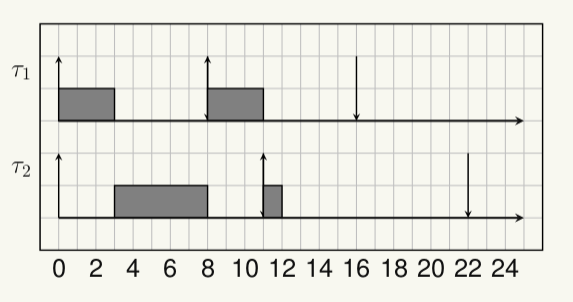
\includegraphics[width = 0.75\textwidth]{images/image14}
    \caption{}
    \label{fig:image14}
\end{figure}

Using EDF the task set is schedulable as seen in figure \ref{fig:image15}
\begin{figure}[!h]
    \centering
    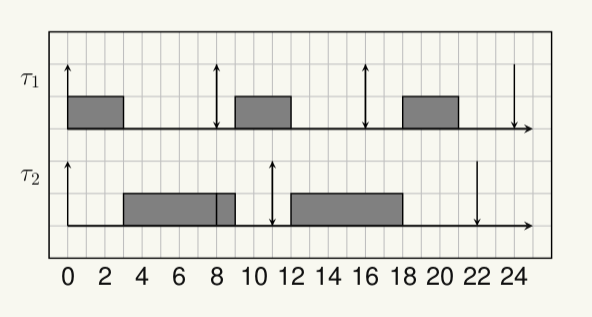
\includegraphics[width = 0.75\textwidth]{images/image15}
    \caption{}
    \label{fig:image15}
\end{figure}

EDF from a theoretically point of view solves all our problems in terms of schedulability, but most real-time operating system utilizes fixed priority assignments.\\
This is because priorities are useful for scheduling analysis and because the priority allows the developer to quantify the relative importance of a task.
